\documentclass[11pt,oneside]{article}

\usepackage[T1]{fontenc}
\usepackage[utf8]{inputenc}
\usepackage{amsmath}
\usepackage{sectsty}
\usepackage{tikz}
\usepackage[labelsep=period,font=small,labelfont=bf]{caption}
\usepackage[charter, cal = cmcal]{mathdesign}
\usepackage[scaled]{helvet}
\usepackage{pdflscape}
\usepackage{afterpage}
\usepackage[hyphens]{url}
\usepackage[colorlinks=true,citecolor=black]{hyperref}
\usepackage{booktabs}

% Highlighted notes
\usepackage{xcolor}
\usepackage{soul}
\newcommand{\note}[1]{\hl{[#1]}}

% Math commands
\DeclareMathOperator{\CVL}{CVL} % CV loss
\DeclareMathOperator{\CINC}{CINC} % CINC function
\DeclareMathOperator{\PRL}{PRL} % Proportional reduction in loss

% Section heading styling
\allsectionsfont{\sffamily}

% BibTeX
\usepackage{natbib}
\bibpunct{(}{)}{;}{a}{}{,}
\renewcommand{\harvardurl}[1]{\textbf{URL:} \url{#1}}

\title{
  Capability Ratios Predict Nothing%
  \thanks{%
    We thank Scott Bennett, Brett Benson, Inken von Borzyskowski, Kevin Clarke, Mark Fey, James Honaker, Zach Jones, Karen Jusko, Holger Kern, David Lewis, Adeline Lo, Matt Pietryka, Marc Ratkovic, Jim Ray, Mark Souva, and Hye Young You for helpful discussions and advice.
    Bryan Rooney provided excellent research assistance.
    We also thank the authors listed in Table~\ref{tab:replications} for making their replication data publicly available.
    The current version of the Dispute Outcome Expectations data can be downloaded from \url{https://dataverse.harvard.edu/dataverse/doe-scores}.
    Replication code and a version history of the project are available at \url{https://github.com/brentonk/crpn}.
  }%
}
\author{%
  Robert J. Carroll%
  \thanks{%
    Assistant Professor, Department of Political Science, Florida State University.  Email:  \nolinkurl{RobCarrollFSU@gmail.com}.
  }%
  \and%
  Brenton Kenkel%
  \thanks{
    Assistant Professor, Department of Political Science, Vanderbilt University.
    Email: \nolinkurl{brenton.kenkel@vanderbilt.edu}.
  }%
}

\begin{document}

\maketitle

\begin{abstract}
  \noindent Modern approaches to political measurement have generally ignored the importance of out-of-sample predictive performance.
  This is problematic for two reasons: first, many of the abstractions scholars attempt to proxy for are themselves expectations; and second, the resulting measures are prone to overfitting.
  We advocate a data-driven approach to measurement focused on out-of-sample prediction.
  We demonstrate the effectiveness of the approach as it applies to proxying the expected outcome of militarized interstate disputes.
  The standard proxy for expected dispute outcomes, the ratio of material capability indices, has almost no predictive power.
  We use ensemble learning to construct a new measure from the same underlying covariates---the Dispute Outcome Expectations score, or DOE---whose predictive power far exceeds that of the standard measure.
  In replications of 18 empirical studies of international relations, we find that replacing standard capability measures with DOE scores usually improves both in-sample and out-of-sample goodness of fit.
\end{abstract}
\thispagestyle{empty}
\newpage
\setcounter{page}{1}


%!TEX root = doe.tex

For all its progress---more nuanced arguments, more useful theories, bigger data and more systematic ways to analyze them---international relations remains, in many ways, a study of power.
This is best reflected in the questions that have endured.
Is the world safer when power is concentrated in a few states or broadly distributed \citep{waltz}?
How does the balance of power between states, or shifts thereof, affect the likelihood of war \citep{organski1980,powell1999,powell2006war}?
Do international organizations allow states to gain benefits they would not receive from power politics alone \citep{keohanenye}?
Without good measures of power, we cannot provide good empirical answers to these fundamental questions.
Consequently, the importance of measuring power to the study of international politics cannot be overstated.

Like many other important concepts in political science, power cannot be measured directly.
Indeed, measurement problems in political science often entail the construction of proxies.
Recent advances in computing and modeling have allowed political scientists to build sophisticated, data-driven proxies for variables as diverse as legislator ideology \citep{clinton2004}, judicial independence \citep{linzer2014}, and country regime types \citep{jackman2008}.
But despite the centrality of power to many important hypotheses in international relations, its measurement has seen far less innovation.\footnote{%
  A recent exception is \citet{Arena:2012}.
}
In this article, we remedy this by devising a new, data-driven approach for measuring power.
Specifically, we aim to learn what combination of observable material capability variables best predicts international dispute outcomes.

We are particularly interested in the crystallization of power that animates the bargaining model of war:  the probability that one state will defeat another in case of militarized conflict, commonly denoted $p$.
This outcome expectation is central to the standard bargaining model \citep{fearon1995}, where it serves as the operationalization of power when dismissing the mutual optimism hypothesis or when unearthing the commitment problem that arises due to shifts in power over time.
The expected outcome of conflict also serves as the main concept of power in \citeapos{Slantchev:2003ka} theory of war termination and in \citeapos{powell2006war} model of commitment problems.
In other words, to study power---at least while motivated by the bargaining model---we must study what shapes dispute outcomes.

We focus on military capabilities as determinants of expected dispute outcomes.
We do so for two reasons.
First, there is a longstanding precedent of starting from the material foundations of power, a practice most commonly associated with historians and theorists in the realist camp \citep{morgenthau,taylor,carr}.
And as \citet[46]{beckley2010economic} observes, even ``[l]iberals and constructivists often conceptualize military power in material terms when refuting its causal significance.''
Second, and of more relevance for the current empirical literature, our focus on the contributions of material capabilities follows the example set by most existing efforts to measure power in the international sphere, starting with the work by \citet{singer1972}.
Most current approaches use the Correlates of War Composite Index of National Capabilities (CINC) score, which combines material factors related to industrialization, wealth, population, and, of course, militarization.

Despite the innovations in measurement in various fields, political scientists have not reached a consensus on what makes for a good proxy, nor is there a common evaluatory metric.
We argue for a predictive criterion:  if the concept of interest is supposed to be associated with some observable outcome, then its proxy should predict the outcome well.\footnote{%
  By prediction, we mean out-of-sample prediction, with data not used to construct the proxy itself.
}
Simple as it may seem, this commitment to prediction highlights important issues.
Like Ulysses or Goldilocks, the proxy maker must strike a delicate balance.
She must learn from the data to construct the measure, else it will fail to capture important dimensions of the concept under study.
\emph{A priori} measures like summed rating scales suffer from this \emph{underfitting} problem, as they fail to take advantage of the wealth of data scholars now possess.
But the analyst who employs a data model for proxy construction faces pitfalls, too.
She may misidentify chance features of her data as systematic, a problem called \emph{overfitting}.
A good proxy should fit the data well, but not so well that it fails to generalize.
An underfit proxy will, of course, be a poor predictor, but so too will a data-driven proxy that maximizes in-sample fit at the expense of generalizability.
Our predictive criterion balances these two considerations.

So too does our methodology.
Supervised learning techniques, having been designed to navigate the straits between underfitting and overfitting, are ideal for data-driven proxy construction.
Machine learning models are flexible enough to analyze relationships far more complex than possible in ordinary regression or measurement models, but they also guard against connecting the dots too aggressively or misinterpreting noise in the data as a complex relationship.
To develop an optimal model for out-of-sample prediction, an analyst simply chooses appropriate tuning parameters, usually by a method like cross-validation that estimates prediction error \citep{Efron:2012es}.
Our approach mirrors that of \citet{Hill:2014ki}, who use cross-validation to assess the relative predictive power of many variables all thought to affect the same outcome.
Our focus, however, is on constructing variables rather than comparing them.

By the predictive criterion, a good measure of relative military power ought to predict dispute outcomes well.
We show that the standard measure, the ratio of CINC scores, predicts militarized dispute outcomes terribly---only 1~percent better than random guessing.
Our new proxy, the Dispute Outcome Expectations (DOE) score, is much better, providing a 20~percent predictive improvement.
It is surprising that the standard measure does so poorly by this criterion, given its ubiquitousness.
As we document below, dozens of recent publications in international relations use CINC-derived measures as proxies for power.
Our use of modern machine learning tools allows us to yield a superior measure from the same data underlying the usual measure.
In addition, the DOE score is interpretable as a probability, just like the bargaining concept of $p$ that animates our approach.

In the course of developing the DOE score, we gain several broad insights about power.
Most fundamentally, material capabilities indeed matter in shaping dispute outcomes, as we explain a substantial amount of variation with a small set of material variables.
This basic result contrasts with previous studies finding no effect of material capabilities \citep{Cannizzo:1980vz,Maoz:1983cw} and reinforces those that conclude capabilities affect victory \citep{wartrap,Stam:1996wl,Sullivan:2012vi}.
We go further to assess which of the CINC components matters most.
Our results suggest that energy consumption is the strongest individual predictor of dispute outcomes.
Surprisingly, military personnel and expenditures matter less on their own.
However, it appears that the effect of these explicitly military components has evolved over the years, while energy consumption's effects have remained more static.

We then go on to demonstrate the DOE score's usefulness to international relations scholars.
We replicate \citeapos{reed2008war} empirical test of Powell's~\citeyearpar{powell1996stability,powell1999} model of the relationship between relative power, the distribution of benefits between states, and the likelihood of conflict.
When we substitute DOE scores in for \citeauthor{reed2008war}'s CINC-based proxy of $p$, the resulting model fits better and predicts better out-of-sample.
More to the point, we extract an important new finding.
Whereas \citeauthor{reed2008war} conclude that the probability of conflict is sometimes greatest between states of equal power---namely, when the distribution of benefits is highly unequal---we find that this is never the case.
The probability of war is always maximized when the state that is worse off under the status quo has a preponderance of power.

Interesting as these results are, it remains that most empirical practitioners only include a capability ratio as a control variable while modeling a wide variety of dependent variables (often the onset of conflict, but sometimes other things).
We take our replication further to see whether the DOE score would be helpful for these scholars as well.
We reanalyze 18 such empirical models to see whether they fit better when we replace the standard proxy with DOE scores.
Since these studies examine outcomes besides the one we use to construct our proxy, there is no guarantee that our new proxy will do better.
Nonetheless, we yield an improvement in fit in 14 of the 18 cases.
In the 14 improved cases, the DOE variables are always jointly significant, whereas the original CINC-based measures of power are jointly insignificant about half the time.
Moreover, in two of these cases the main substantive hypothesis is no longer supported in the replicated model.
We thereby show how using a poor proxy for relative power, even as a control variable, can lead scholars to understate the impact of military power and to reach conclusions not supported by the data.

The paper proceeds in five sections.
In the first, we lay out our general argument about proxy construction and its application to the case of military power.
Section~\ref{sec:methods} describes the data and methods we use to construct a new proxy for expected dispute outcomes.
In Section~\ref{sec:scores}, we discuss the advantages and disadvantages of our measure.
Section~\ref{sec:replications} contains the results of our replications and advice for using the DOE score.
The final section addresses next steps and concludes.

%%% Local Variables:
%%% mode: latex
%%% TeX-master: "doe"
%%% End:



\section{Predictive Power and Proxy Variables}

We are often interested in questions that link observed data to some unobserved quantity.
This latter quantity may be unobserved because it is difficult (or impossible) to measure directly (like wealth) or because it is an abstraction (like the ideal point of a voter in a spatial model).
In either case, the applied analyst faces a choice between omitting some potentially important variable and including some proxy variable in its stead \citep{stahlecker1993}.
There is no best choice: some theoretical econometricians \citep[e.g.][]{mccallum1972} argue for the inclusion of all proxies (including crude ones), while others \citep[e.g.][]{maddala1977} support only the use of reliable proxies.
Even those in the former camp, however, admit that reliable proxies perform better than unreliable ones.

Healthy disciplines use good measures for central concepts \citep{kuhn1977}, and so social science progresses, in part, by developing better ways to construct proxy variables.\footnote{Here we focus on the importance of models in producing measures; equal weight should be assigned to advances in the estimation of these models' relevant parameters, most notably to advances in Bayesian estimation \citep{jackman2001,martin2002,clinton2004,bafumi2005}.}
Much recent progress is due to the development of measurement models.\footnote{Of course, the use of theory in the act of measurement is nothing new.
  Economics retains its longstanding commitment to structural estimation whereby theoretical models are used to uncover relevant quantities.
  For current applications to the structural estimation of dynamic discrete-choice games (for example), see \citet{su2012} and \citet{egesdal2013}.} \citet[2]{jacoby2014} observes:
\begin{quote}
  ``All of us are comfortable with the notion of statistical \emph{models} that provide representations of structural relationships between variables.  But, modern social science also regards measurement as a model that pertains to each of the individual variables.  Careful attention and rigorous approaches are just as important for the latter type of models, as they are for the former.''
\end{quote}
Moreover, when the unobserved quantity is an abstraction, appropriate measurement models allow the analyst to perform direct tests that follow from the same set of assumptions as those used in the original, theoretical model.
As \citet[355]{clinton2004} put it in the context of testing legislative behavior, ``it is inappropriate to use ideal points estimated under one set of assumptions...to test a different behavioral model....''  \citet[530]{shor2011} note that the close relationship between statistical and theoretical models of legislative behavior (and their requisite assumptions) ``has contributed to a much tighter link between theory and empirics in these subfields of political science.''

While better models (and better ways to estimate their parameters) have improved our measures of a variety of important quantities, it remains problematic that modern political measurement has ignored the importance of predictive power in producing proxies.
This is odd, as seminal contributions to the literature utilize classification---a criterion often used in machine learning, where the focus is usually on prediction---as a way to prove a new measure's superiority over extant ones. For example, in the classic paper on ideal point estimation in American legislatures, \citet[Table 3]{poole1985} report that a simple classification approach based on their NOMINATE scores correctly predicts over 80\% of legislative votes in most years in their data. Though their procedure estimates ideal points via the method of maximum likelihood rather than via a classification criterion, it remains that this analysis lies prone to textbook overfitting problems.
In their paper, Poole and Rosenthal estimate ideal points within a single Congressional session, and their classification test then uses those ideal points to assess voting within the same Congressional session.
While many of the correct classifications reflect the spatial model's explanatory virtues, others may arise due to overfitting to the data within that Congressional session.

It is for these reasons that we advocate a data-driven approach based on predictive performance.  While traditional statistical approaches to measurement minimize error or maximize likelihood within the entire data set, we instead aim to optimize out-of-sample prediction.\footnote{Our formal criterion for predictive performance, the log loss function, is explicitly described in the methods section.}
We do so through cross-validation.
Each observation in our data is assigned to a ``fold,'' and each fold is given a battery of predictions based on models fit to data not including the fold.  
That is, each observation is assigned a set of predictions from models fit to other data.
Our battery of predictions include a variety of estimators, including traditional models like ordered logit but also more flexible algorithms like random forests or averaged neural nets. 
We determine the best weighted average of these estimators by using the out-of-sample predictions assigned to each observation.
With models fit, predictions assessed, and weights derived, we use the results to produce a final estimate.

This approach explicitly addresses the problems enumerated above: it avoids the overfitting problems associated with traditional measurement techniques and the model selection problems associated with attempts to bring new data to bear for predictive purposes.
We believe that the costs of our approach---additional computation and difficulty in interpreting the results---pale in comparison to these benefits.

%%% Local Variables:
%%% mode: latex
%%% TeX-master: "doe"
%%% End:



\section{The Capability Ratio and Its Discontents}

Thanks in part to the popularity of formal models of choice under uncertainty, many unobserved quantities like those discussed above take the form of probabilities.
Our application---expectations about war outcomes as parameterized by some probability $p \in [0,1]$---is no different.
We want to create a proxy for the chance that Country~A would prevail in a dispute against Country~B, given their observable characteristics, $x_A$ and $x_B$.
Since a measure of a probability must lie within the unit interval, a natural way to proceed is to propose an indexing function $g$, where $g(x) \geq 0$, and then take the ratio of indices,
\begin{equation}
  \label{eq:ratio}
  f(x_A, x_B)
  =
  \frac{g(x_A)}{g(x_A) + g(x_B)}.
\end{equation}
The quality of such a measure depends on both the selected characteristics and on the appropriateness of the indexing function~$g$.
This latter responsibility plays a large role in the development of good measures and is our primary area of focus.

Though simple, this enhanced ratio-based approach is remarkably powerful and finds use in a diverse array of applications.
A classic success comes from the study of baseball outcomes, where the Pythagorean prediction \citep{james1983,miller2007} of a team's winning percentage is defined as
\begin{align*}
  f\left(\text{Runs Scored}, \text{Runs Allowed} ; \alpha\right) &= \frac{\text{Runs Scored}^\alpha}{\text{Runs Scored}^\alpha + \text{Runs Allowed}^\alpha},
\end{align*}
where $\alpha \geq 0$ adjusts $x$'s shape.
Here the quest for the best-fitting $g$ amounts to estimating $\alpha$; \citet{james1983} originally proposed $\alpha = 2$ \emph{ad hoc}, and later analysts found that $\alpha = 1.83$ fit the data best.
Though the analyses that produced this estimate suffer from the overfitting problems discussed above, the Pythagorean predictor still performs quite well when imposed upon out of sample data.

% TODO: Some of this notation collides with what we use for multiple imputation in the appendix.  Do we care?

When proxying for expected dispute outcomes, empirical conflict scholars normally use transformations of data on states' material capabilities.
We now relate the typical transformation to our discussion of ratio-based measures above.
We begin by introducing some helpful notation: call the set of states $\mathcal{I} = \left\{1, \ldots, I\right\}$; the set of variables $\mathcal{J} = \left\{1,\ldots,J\right\}$; and the set of years $\mathcal{T} = \left\{1,\ldots, T\right\}$.
Denote state $i$'s value for variable $j$ in time $t$ as $M_{ijt}$.
The set of all data is $M$, and all data in year $t$ is $M_t$.
Define state $i$'s share of variable $j$ in year $t$ as
\begin{align*}
  S_{ijt}(M_{t}) &= \frac{M_{ijt}}{\sum_{\mathcal{I}} M_{ijt}}.
\end{align*}

We now introduce the \emph{CINC function}.\footnote{Here CINC stands for ``Composite Index of National Capability'' as given in the Correlates of War National Material Capabilities data \citep{singer1972}.}
State $i$'s CINC score in year $t$ is its average share across all variables:
\begin{align*}
  \CINC_i(M_t) &= \frac{\sum_{\mathcal{J}} S_{ijt}}{\left|\mathcal{J}\right|}.
\end{align*}
State $i$'s CINC score therefore falls in $[0,1]$.
The CINC score is the ``most commonly used measure'' of power in empirical conflict studies \citep[212]{kadera2004}.

Following the discussion in the previous section, the most intuitive CINC-based proxy for $p$ is a na\"{\i}ve \emph{capability ratio}:
\begin{align*}
  f_{\text{CR}}(M_t) &= \frac{\CINC_A(M_t)}{\CINC_A(M_t) + \CINC_B(M_t)}.
\end{align*}
Our approach, then, makes explicit the fact that $\CINC$ is simply a candidate $g$ function imposed upon annual material capability data $M_t$.

Problems emerge immediately.
Two of these pertain to the CINC function itself.
First, as has been documented, the CINC function is sensitive to changes in state membership over time \citep{organski1980,gleditsch1999,kadera2004}.
Second, the CINC function's equal weighting of all indicators is entirely \emph{ad hoc}.
For example, the CINC function assigns the same importance to military spending as it does to personal energy consumption.
Whether this is an appropriate assignment is an empirical question that goes unanswered.
Even on the tenuous assumption that $\CINC$ is a good data reduction technique on $M_t$, it is not clear whether it serves as a good $g$ function.
Prior to entering $f_{\text{CR}}$, should the CINC scores be exponentiated given some parameter on returns to scale, or perhaps instead logged?
Finally, even given that $\CINC$ is a useful index, we do not know whether a ratio-based approach is appropriate at all.
In other words, taking the capability ratio at its word requires making a host of assumptions that may not hold well enough to make it useful in applications.\footnote{
  It is worth noting that some applications follow \citet{bremer1992} in using the explicit CINC ratio:
  \begin{align*}
    f_{\text{Bremer}}(M_t) &= \frac{\max\left\{\CINC_A(M_t),\CINC_B(M_t)\right\}}{\min\left\{\CINC_A(M_t),\CINC_B(M_t)\right\}}.
  \end{align*}
  Bremer's approach does not fall in $[0,1]$, though it could be transformed through a logit or probit CDF.
  However, it is a monotonic transformation of the aforementioned capability ratio, and it suffers from similar problems anyway.
}

Yet it is widely used. Capability ratios (or similar manipulations of CINC scores) feature prominently in many recent empirical studies in international relations.
As we might expect given the importance of the bargaining model, many of these \citep[e.g.][]{gartzke2007,salehyan2008} use capability ratios in regressions predicting the onset of a militarized interstate dispute.
Still others focus on particular features of a militarized interstate dispute, such as the nature of its termination \citep{beardsley2008} or whether its combatants complied with laws of war \citep{morrow2007}.
Still other studies focus on other phenomena not directly related to disputes, such as the onset of sanctions \citep{whang2013}, issue agreements \citep{mitchell2007}, or nuclear assistance provisions \citep{kroenig2009}.
A more exhaustive survey of the use of capability ratios is beyond the scope of this paper, but suffice it to say that it is the go-to measure of relative power in international relations.

One might politely defend the capability ratio by noting that it asks the $\CINC$ function to perform a job it was not designed for.
We would agree.
It is worth noting, however, that early proponents of the $\CINC$ function \citep[24]{singer1972} sought to understand how ``uncertainty links[s] up with capability patterns on the one hand and with war or peace on the other.''
Writing over two decades before the classic introduction to the bargaining model of war \citep{fearon1995}, these authors lacked the abstract target---$p$---that we currently have, but their enterprise was largely similar.
Though their focus on systemic, rather than dyadic, patterns reflects the dominant flavor of realism at the time, they still wanted to know how preponderance of power related to the decision to fight.
So, while it remains true that the capability ratio is not meant to directly relate to $p$ in a bargaining model, it \emph{was} meant to tell us something about how uncertainty relates to war.

Remedying these problems by fitting a model---perhaps estimating an exponent on the CINC scores in $f_{\text{CR}}$, or weights for the CINC indicators---would be a laudable first step, but it would still suffer from functional form dependencies.
The careful scholar might sidestep these by fitting an ensemble of models with different functional forms imposed, but so long as the ensemble is fit to the entire capability data set, it will suffer from overfitting and lose predictive power.
In the next section, we outline our method for estimating $p$ that suffers neither from overfitting nor from pathologies in the $\CINC$-utilizing, ratio-based approach.

%%% Local Variables:
%%% mode: latex
%%% TeX-master: "doe"
%%% End:



\section{Building a Better Proxy for Expected Dispute Outcomes}
\label{sec:methods}

Our goal now is to squeeze as much predictive power as we can from data on states' material capabilities.
When prediction is the goal, ``black box'' algorithmic techniques usually outpace standard regression models \citep{Breiman:2001fd}.
So, to build our new measure, we augment traditional approaches with methods from machine learning.

\subsection{Data}

To evaluate the predictive performance of the capability ratio and then to build an alternative measure, we use data on the outcomes of international disputes.
We combine the National Material Capabilities data \citep{singer1972} with information on the outcomes and participants of Militarized International Disputes between 1816 and 2007 \citep{Palmer:2015hp}.
Our data consist of $N = 1{,}740$ disputes, each between an ``initiator,'' or Country~A, and a ``target,'' or Country~B.\footnote{
  See the Appendix for the data construction and coding specifics.
}
Every dispute outcome is either A~Wins, B~Wins, or Stalemate, which we denote by $Y_i \in \{A, B, \emptyset\}$, respectively.
Most disputes end in a stalemate, and victory by the initiator is more than twice as likely as victory by the target, as shown in Table~\ref{tab:mid}.

\begin{table}[htp]
  \centering
  \input{tab-mid}
  \caption{
    Distribution of the three dispute outcomes.
  }
  \label{tab:mid}
\end{table}

We model dispute outcomes as a function of the participants' military capabilities.
Our data source, the National Material Capabilities dataset, records annual observations of six characteristics of a country's military capability: military expenditures, military personnel, iron and steel production, primary energy consumption, total population, and urban population.\footnote{
  There are missing observations in the National Material Capabilities data.
  Consequently, about 17~percent of the disputes we observe contain at least one missing cell.
  We use multiple imputation to deal with missingness \citep{honaker_what_2010}; see the Appendix for details.
}
We also calculate each country's share of the global total of each component, giving us 12 variables per dispute participant.
The matrix of predictors has 26 columns: the 24 individual capability characteristics of the initiator and target, the standard capability ratio, and the year the dispute began.
The values of these predictors for the $i$'th dispute are collected in the vector $X_i$.

\subsection{A Metric for Predictive Power}

We face two challenges in evaluating a model's predictive power.
The first is to define a metric for predictive power---one that is appropriate to the task at hand and reasonably interpretable.
The second is to measure each model's ability to predict \emph{out of sample}.
Our main purpose, which is to measure the chances of victory for each side in a hypothetical interstate dispute, is inherently an out-of-sample prediction task.
We do not want a model that overfits the sample data at the expense of its predictive power when brought to new data.

As fortune plays a role in every military engagement, it would be impossible to perfectly predict the outcome of every dispute.
We therefore want a measure of predictive power that respects the probabilistic nature of militarized disputes.
Classification metrics like the accuracy statistic, also known as the percentage correctly predicted, do not fit the bill.
Instead, we employ the log loss, which is the negative of the average log-likelihood, as our metric for predictive power \citep[221]{Hastie:2009wpa}.
Let a \emph{model} be a function $\hat{f}$ that maps from the dispute-level predictors $X_i$ into the probability of each potential dispute outcome, $\hat{f}(X_i) = (\hat{f}_A(X_i), \hat{f}_B(X_i), \hat{f}_{\emptyset}(X_i))$.
The ``hat'' on $\hat{f}$ is there to emphasize that the form of the function has been learned from the data, whether by estimating regression coefficients or by a more flexible predictive algorithm.
The log loss of the model~$\hat{f}$ on the data~$(X, Y)$ is\footnote{
  To avoid numerical problems, very low probabilities are trimmed at $\epsilon = 10^{-14}$.
}
\begin{equation}
  \label{eq:log-loss}
  \ell(\hat{f}, X, Y)
  =
  - \frac{1}{N} \sum_{i = 1}^{N} \sum_{t \in \{A, B, \emptyset\}}
  \mathbf{1} \{Y_i = t\} \log \hat{f}_t(X_i).
\end{equation}
Smaller values of the log loss represent better predictive power, with the lower bound of~$0$ indicating perfect prediction.

We care mainly about the generalization error of our models---the expected quality of their predictions for new data that was not used to fit the models.
Our small sample size of $N = 1{,}740$ makes this tricky.
If we had a surplus of observations, we could use some suitably large number to fit our models and hold out the remainder to assess the models' predictive power.
But with as little data as we have, splitting the sample is ill-advised: we cannot hold out enough observations to estimate the generalization error precisely without harming the precision of the model itself.
So, to measure out-of-sample predictive power without losing data, we turn to $K$-fold cross-validation \citep[241--249]{Hastie:2009wpa}.
We randomly assign each dispute observation to a ``fold'' $k \in \{1, \ldots, K\}$, where we follow standard practice by setting $K = 10$.\footnote{Standard practice here stands on firm ground; \citet{molinaro2005} find that 10-fold cross-validation performs quite similarly to leave-one-out cross validation (the ``ideal case'' for cross-validation) without having to take on massive computational costs.  10-fold cross-validation also performs better than the .632+ bootstrap, split-sample techniques, and Monte Carlo cross-validation, particularly in smaller samples like ours.}
For each~$k$, we split the data into a ``test'' sample containing fold~$k$ and a ``training'' sample containing the remainder of the data.
We fit a model only on the training sample and then calculate its predicted probabilities for the data in the test sample.\footnote{
  \label{fn:nested-cv}
  When dealing with models with tuning parameters that are themselves selected by cross-validation, we choose tuning parameters separately within each of the $K$ iterations via another cross-validation loop.
  This nested cross-validation is necessary to keep our estimates of generalization error from being too optimistic \citep{Varma:2006ch}.
}
After repeating this $K$ times, we have an out-of-sample prediction for each observation in our data---one that was calculated from a model that did not see the observation in question.
We compare these predicted probabilities to the observed outcomes to estimate our models' generalization error.
Formally, the cross-validation loss of the model~$\hat{f}$ is the average out-of-fold log loss,
\begin{equation}
  \label{eq:cv-loss}
  \CVL(\hat{f})
  =
  \frac{1}{K} \sum_{k=1}^K \ell \left(
    \hat{f}^{(-k)}, X^{(k)}, Y^{(k)}
  \right),
\end{equation}
where $(X^{(k)}, Y^{(k)})$ is the data in the $k$'th fold and $\hat{f}^{(-k)}$ is the model~$\hat{f}$ fit to the data excluding the $k$'th fold.

Because it is measured on the log-likelihood scale, the log loss metric is hard to interpret on its own.
To ease the interpretation, we compare models' log loss to that of a null model, whose predicted probabilities always equal the sample proportions of each outcome.
The proportional reduction in cross-validation loss of the model~$\hat{f}$ is
\begin{equation}
  \label{eq:prl}
  \PRL(\hat{f})
  =
  \frac{
    \CVL(\hat{f}_{\text{null}}) - \CVL(\hat{f})
  }{
    \CVL(\hat{f}_{\text{null}})
  }.
\end{equation}
The theoretical maximum, for a model that predicts perfectly, is~$1$.
If a model predicts even worse than the null model---meaning, in essence, it is worse than random guessing---its proportional reduction in loss is negative.

\subsection{Modeling Dispute Outcomes}

Our task now is twofold: to assess the predictive power of the capability ratio and, should we find it lacking (as we do), to build a better alternative.

We model dispute outcomes as a function of the capability ratio via ordered logistic regression \citep{McKelvey:2010gv}.
To reduce skewness, we take the natural logarithm of the capability ratio.
The parameter estimates from the capability ratio model on the full sample appear in Table~\ref{tab:capratio}.
Although these results do not speak directly to the capability ratio's out-of-sample performance, they foreshadow why its predictive power is so limited.
The coefficient on the capability ratio is statistically significant but small relative to the cutpoints, indicating a substantively weak relationship.
Dividing the cutpoints by the coefficient, we see that we would need a logged capability ratio below $-13$ or above $+7$ to predict any outcome other than a stalemate.
These bounds lie well outside the observed range of capability ratios in the dispute data, which are bounded below by $-9.1$ (Palau--Philippines 2000) and above by $-0.0004$ (Germany--Panama 1940).
In other words, the capability ratio always predicts a stalemate within the sample.
This does not bode well for its out-of-sample performance.

\begin{table}[tp]
  \centering
  \input{tab-capratio}
  \caption{
    Results of an ordered logistic regression of dispute outcomes on the capability ratio using the training data.
    Because there are no missing values in the CINC scores, these estimates are identical across imputed datasets.
  }
  \label{tab:capratio}
\end{table}

We want a better model than what the capability ratio gives us, but we do not have a strong \emph{a priori} sense of what the data-generating process---the true relationship between material capabilities and dispute outcomes---looks like.
So we use tools from machine learning that are designed to predict well without imposing much structure on the data.
Ideally, we would select the predictive model that is best for our data, but there are too many algorithms to try them all.
To narrow it down, we defer to the machine learning experts on which algorithms are best.
We draw our set of candidate models from the top-ten list by \citet{Wu:2007ev} and from the best performers in the tests by \citet{FernandezDelgado:2014ul}.
After excluding those unsuited to our data,\footnote{
  Four of the algorithms named in \citet{Wu:2007ev}---$k$-means, Apriori, expectation maximization, and PageRank---are not suited for the prediction task at hand.
  We also excluded AdaBoost due to long computation time and naive Bayes due to poor performance in initial tests.
}
we end up with six predictive algorithms to try: C5.0, support vector machines, $k$-nearest neighbors, classification and regression trees, random forests, and ensembles of neural nets.\footnote{
  See the Appendix for full details of each method.
}
Each algorithm is widely used for prediction and can predict dispute outcome probabilities as a complex, potentially nonlinear function of the material capability components.
As a compromise between these flexible ``black box'' models and the rigid capability ratio model, we also test ordered logistic regression models on the capability components.

In the spirit of flexibility, we try each model with different sets of predictors from the capability data.
We examine four sets of variables: the raw capability components and the annual component shares, each with and without the year the dispute began.
All of our models allow for interactive relationships, so including the year of
the dispute lets the effect of each capability component vary over time.
With two sides per dispute and six capability variables per side, each model has 12 or 13 variables, depending on whether the year is included.
All told, we have 30 candidate models: four sets of variables for each of our seven algorithms, plus the capability ratio model and a null model used as a baseline.

We use cross-validation to estimate how well each of our candidate models predicts out of sample.
The final problem, once we have the cross-validation results, is to choose a model---the one we will use to construct an alternative to the capability ratio as a measure of expected dispute outcomes.
It is tempting to simply pick the model with the lowest cross-validation loss.
We can do even better at prediction, however, by taking a weighted average of all the models.
We use the super learner algorithm \citep{vanderLaan:bz} to select the optimal model weights via cross-validation.
Given a set of $M$ candidate models $\hat{f}_1, \ldots, \hat{f}_M$, we select weights $\hat{w}_1, \ldots, \hat{w}_M$ to solve the constrained optimization problem
\begin{equation}
  \label{eq:super-learner}
  \begin{aligned}
    \min_{w_1, \ldots, w_M}
    &\quad
    \CVL \left(
      \sum_{m=1}^M w_m \hat{f}_m
    \right)
    \\
    \mbox{s.t.}
    &\quad
    w_1, \ldots, w_m \geq 0,
    \\
    &\quad
    w_1 + \ldots + w_m = 1,
  \end{aligned}
\end{equation}
Our final model is the super learner, $\hat{f} = \sum_m \hat{w}_m \hat{f}_m$.
Each individual model is a special case of the super learner, with full weight $\hat{w}_m = 1$ placed on a single $\hat{f}_m$.
Hence, by the cross-validation criterion, we should prefer the super learner over any individual model.\footnote{
  \label{fn:sl-bias}
  As usual when selecting tuning parameters via cross-validation, the value of equation~\eqref{eq:super-learner} is not an unbiased estimate of the generalization error of the super learner.
  Nested cross-validation is computationally infeasible for the super learner, so we calculate the bias correction recommended by \citet{Tibshirani:2009tz} to estimate its generalization error.
}  That said, the super learner does provide the capability ratio with an opportunity to defend itself; should it earn a high weight, then our costly enterprise may not be worth the effort.

To summarize, we fit and cross-validate $M = 30$ candidate models, then combine them into a super learner that we will use to construct a better proxy for expected dispute outcomes.
The biggest downside of our approach is that the results are not easily interpretable.
Because the super learner entails averaging a large set of models---some of which, like random forests, are themselves difficult to interpret---it gives us no simple summary of how each predictor affects dispute outcomes.
This is not a problem, given our aims.
Certainly, we would not recommend the super learner as a means of testing hypotheses about the determinants of dispute outcomes.
However, our goal is not to test a hypothesis---it is to construct the best proxy possible for how a dispute between two countries is likely to end.
In this context, it is worth sacrificing interpretability for the sake of predictive power.

\subsection{Results}

We now turn to the cross-validation results, which are summarized along with the super learner weights in Table~\ref{tab:ensemble}.
As the in-sample analysis hinted, the capability ratio is indeed a poor predictor of dispute outcomes.
Its proportional reduction in loss is~0.01, which means its predicted probabilities are just 1~percent more accurate than the null model.
This number is not encouraging, but what matters even more is whether we can do better.
A glance at Table~\ref{tab:ensemble} confirms that we can: all but one of our 27 alternative models has greater predictive power than the capability ratio, many of them considerably better.
With these results in hand, we feel comfortable dismissing the capability ratio as a suboptimal proxy for expected dispute outcomes.

\begin{table}[tp]
  \centering
  \input{tab-ensemble}
  \caption{
    Summary of cross-validation results and super learner weights.
    All quantities represent the average across imputed datasets.
  }
  \label{tab:ensemble}
\end{table}

We can glean a few basic intuitions about the relationship between capabilities and dispute outcomes from the cross-validation results.
First, the relationship is too complex to capture in a linear model.
The best of our ordered logits has a 10~percent proportional reduction in loss, about half that of the best nonlinear model (the neural net ensemble on capability components with year included).
So we cannot fix the problems with the capability ratio just by disaggregating it into its component parts.
Second, the capability--outcome relationship changes over time.
Accounting for the year of the dispute improves our models' predictive power: in 13 out of 14 cases, the model that includes time predicts better than its time-less counterpart.\footnote{
  The difference in log loss is statistically significant (paired $t = -3.25$, $p = 0.006$).
}
Unlike the capability ratio, flexible predictive algorithms can capture this variation.
Finally, the models trained on the raw capability components tend to outperform those trained on the annual shares of components.\footnote{
  The difference in log loss is statistically significant (paired $t = -3.14$, $p = 0.008$).
}
This runs contrary to way the CINC score is constructed---it is an average of capability shares---suggesting another reason why the capability ratio is such a poor predictor.

As we expected, the super learner ensemble performs better than any of the candidate models from which it is constructed.
The ensemble's proportional reduction in loss is about 23~percent, or four percentage points better than the best candidate model.
Even after we apply a bias correction (see footnotes~\ref{fn:nested-cv} and~\ref{fn:sl-bias}), the super learner's predictive power is still the best among our models.
Looking at the weights, what stands out is how few models are substantial components of the super learner: just five models have a weight of at least 5~percent.
More generally, while models with lower generalization error tend to receive more weight, the relationship is by no means one-to-one.
We see this because the ensemble prefers not only predictive power, but also diversity.
Different classes of models have different blind spots; the more diverse the ensemble is, the more these blind spots are minimized.
A model that looks bad on its own might still merit non-negligible weight in the optimal ensemble if it captures a slice of the data missed by the models that are best on their own.

\begin{figure}[tp]
  \centering
  \input{fig-oof-pred}
  \vspace{-2em}
  \caption{
    Ternary plots of out-of-fold predicted probabilities according to the capability ratio model and the super learner.
    Each predicted probability is calculated by fitting the model to 9/10 of the data, not including the observation in question---an approach that simulates true out-of-sample prediction.
  }
  \label{fig:oof-pred}
\end{figure}

The super learner predicts dispute outcomes much better than the capability ratio does.
As we have just shown, the capability ratio only improves by~1~percent on a null model, whereas the super learner gives a~20~percent improvement.
For another illustration of the difference in predictive power, see the plots of out-of-fold predicted probabilities---the ones we use in cross-validation---in Figure~\ref{fig:oof-pred}.
Under the capability ratio model, all but a handful of disputes are predicted to have an 80--90~percent chance of ending in stalemate.
Seeing how narrow the capability ratio's predictive range is, it is little surprise that it barely does better than a null model at prediction.
Conversely, the super learner makes much better use of the material capability data.
Its predictive range is greater, which in turn allows it to achieve a stronger---though hardly perfect---relationship between predicted and observed outcomes.

What should we make of the fact that, even after all this predictive effort, about 80~percent of the variation in dispute outcomes remains unexplained?
One problem is that our sample size is too small to fit flexible models without a loss of precision.
For the sake of precise predictions---though not that of humankind!---it would be better to have far more dispute observations to use for model building.
The bigger issue, however, is that material capabilities do not tell the whole story.
No matter how many modeling tricks we pull out, we cannot change the fact that militarized dispute outcomes depend on much more than raw capabilities.
Some of these other predictors, like the distance between the disputants, are easily measured; others, like the cleverness of their leaders, are not.
In principle, it is possible to incorporate additional variables (at least those that can be quantified) into the super learner to attain even better outcome predictions.
That goes beyond the scope of this paper, which only aims to show how we can best use the data underlying the capability ratio.

%%% Local Variables:
%%% mode: latex
%%% TeX-master: "doe"
%%% End:



\section{The New Measure: Dispute Outcome Expectations}
\label{sec:scores}

We use the super learner results to construct a new proxy for expected dispute outcomes---one that predicts actual dispute outcomes much more accurately than the capability ratio does.
For any pair of countries at a particular point in time, whether or not they actually had a dispute with each other, we can use the super learner to ask, ``Based on what we know about their material capabilities, how would a dispute between these countries be likely to end?''
To construct the new proxy, we use the super learner to make predictions for every directed dyad--year in the international system between 1816 and 2007, the range of years covered by the National Material Capabilities data.
We call the resulting dataset the Dispute Outcome Expectations data, or DOE.
The DOE data contains predictions for more than 1.5~million directed dyad--years.\footnote{%
  About 19~percent of directed dyad--years contain missing values of the capability components for at least one country.
  We average across imputations of the capabilities data to calculate the DOE scores for these cases.
  See the Appendix for details.
}

The DOE scores are naturally directed, since each dispute in our training data contains an initiating side and a target side.
However, many analyses in the international conflict literature (e.g., of dispute occurrence) use undirected data.
We calculate undirected DOE scores through a simple average of the directed values.
For example, to calculate the probability that the United States would win a dispute against the United Kingdom in 1816, we average its estimated chances of victory as an initiator (36~percent) and as a target (11~percent) to yield 23.5~percent.
If an analyst using the DOE data believed that the likely identity of an initiator in a hypothetical dispute were not a coin flip, she could take a different average of the directed scores to produce a more representative undirected score.

The DOE measures have two advantages over the capability ratio as a proxy for expected dispute outcomes.
First, they are direct measures of the quantity of primary interest to scholars of conflict: the probability that each state would win in a hypothetical dispute.
Although the capability ratio is a proportion, it cannot be interpreted as the probability of victory.
The ease of interpretation is particularly important for scholars who wish to control for expected dispute outcomes in a regression model.
The coefficient on a DOE score can be interpreted directly as the marginal effect of a state's chance of victory; the coefficient on the capability ratio cannot.
Second, as we have already seen, within the set of state pairs where disputes occur, the DOE measures are much better predictors of the outcome than the capability ratio is.
In short, they are superior proxies, and therefore are the appropriate choice for scholars who need an accurate measure of expected dispute outcomes.
The canonical correlation between the DOE scores and the capability ratio is 0.44 (for both the directed and undirected DOE scores), so the measures are related but distinct.

The DOE scores have one drawback worth mentioning: they should not be included as controls in regressions whose dependent variable is the outcome of a dispute or war.
This may seem contradictory, given how much effort we have just spent showing that DOE scores are superior predictors of dispute outcomes.
The reason they are superior is that, unlike the capability ratio, they are calibrated using real dispute data.
But this in turn means that DOE scores would be endogenous in a regression whose dependent variable is dispute outcomes---i.e., the same data we used to construct the DOE scores.
Another way to think about it is that the DOE score measures expectations of dispute outcomes, and there is no reason to think these expectations themselves have an independent effect on the outcomes.
So when we test causal hypotheses about dispute outcomes, we should control for raw capabilities, not expectations.
But when we are modeling dependent variables that might be affected by expectations, such as the onset of a crisis or a state's decision to join an ongoing conflict, we should use the best available proxy for those expectations---namely, the DOE scores.

\begin{figure}[tp]
  \centering
  \input{fig-vs}
  \vspace{-2em}
  \caption{
    Comparison of predicted outcome probabilities over time from the capability ratio and the super learner (DOE scores) for the United States versus Russia.
    These plots use the undirected scores.
  }
  \label{fig:vs}
\end{figure}

To illustrate the contrast between the capability ratio and DOE scores for forecasting hypothetical dispute outcomes, Figure~\ref{fig:vs} plots the two models' predictions over time for the United States versus Russia.
According to the capability ratio model, there was essentially no change between 1816 and 2007 in the likelihood of either side winning a dispute.
We need not dwell on the implausibility of this prediction.
Conversely, the DOE scores stack up with our intuitions relatively well: the predicted chance of a stalemate balloons during the Cold War, but the chance of victory by the United States picks up afterward.

In light of the DOE scores' superior predictive performance in the Militarized Interstate Disputes data, we are inclined to believe they dominate the capability ratio as a proxy for expected dispute outcomes.
Next, we test this conjecture by seeing if replacing the capability ratio with DOE scores in empirical models of international conflict improves their in-sample fit and out-of-sample predictive power.

%%% Local Variables:
%%% mode: latex
%%% TeX-master: "doe"
%%% End:



%!TEX root = doe.tex

\section{Using the New Measure}
\label{sec:replications}

\note{Will need to rewrite this once the Reed stuff is in.}

We have shown that our measure, the DOE score, predicts international dispute outcomes better than the capability ratio.
But most recent studies of conflict do not aim to predict how disputes will end.
They focus on other dependent variables, and they usually only treat the capability ratio (or other functions of raw capabilities) as a control.
In this section, we investigate how well the DOE score performs as a replacement for the capability ratio in this more typical setting.
First, we replicate 18 recent empirical models of various international phenomena, finding that these models usually fit and predict better when we replace CINC-based measures with DOE scores.
After that, we provide some advice to practitioners on how to decide which measure---or measures---to include.

\subsection{What's New about Power?}

The DOE score's greatest potential lies in its ability to enhance tests of the role of power in international relations.
To that end, we begin our replication analysis by replicating a well-known test of the bargaining model.

\citet{reed2008war} provide an empirical examination of the bargaining model developed by \citet{powell1996stability,powell1999}.
The analysis focuses on two important parameters:  the probability that one state would prevail over the other in a conflict, $p$, and the distribution of benefits between the two states, $q$.
For example, $q$ may capture where a border is drawn between two neighboring states, though this animation is not necessary.
\citet[258]{powell1996stability} derives\footnote{%
  The probability here is equivalent to Powell's but uses the same expression as Reed et al. to simplify explication.
}
the equilibrium probability of conflict as
\begin{align*}
  \pi(p, q) &= \begin{cases}
  |q - p| - (q - p)^2, & |q - p| \leq \frac{1}{2} \\
  \frac{1}{4}, & |q - p| \geq \frac{1}{2}
  \end{cases},
\end{align*}
and Reed et al. provide a direct test of this expression by incorporating proxies of $|q - p|$ and $(q - p)^2$ (lagged one year) into a model of dispute onset.
They develop a new measure of $q$ based on United Nations roll call votes, and their measure of $p$ is a normalized cousin of the capability ratio based on the differences in CINC scores.\footnote{%
  For details on their measure of $p$, see footnote 11 of \citet[1211]{reed2008war}.
}
Our goal here is to replicate their results and then to estimate a faithful parallel model that uses DOE scores, rather than CINC scores, to proxy for $p$ while keeping all other covariates, including the Reed et al. measure of $q$, the same.

The first task is to assess the similarities of the two proxies of the two variables.
We plot the kernel densities of the measures in Figure \ref{fig:rcnw-measures}.
\begin{figure}[!ht]
  \centering
  \input{fig-rcnw-measures.tex}
  \caption{Comparison of Reed et al. (2008) and DOE proxies of $|q - p|$ and $(q - p)^2$.}
  \label{fig:rcnw-measures}
\end{figure}
Here the left column depicts $|q - p|$ and the right column depicts $(q - p)^2$.
The reader will note that the distributions are generally very similar, with nearly identical extrema, centralities, and dispersions.
The two absolute differences correlate at around~0.962, while the two squared differences correlate at around~0.957.
The average difference in the $|q - p|$ measures is~$-0.009$, and the average difference in the $(q-p)^2$ measures is~$-0.008$.
Suffice to say, the DOE versions of the two power variables are quite similar to those employed by Reed et al., which is not all that surprising given that we are using the same measure of $q$ for their construction.

Despite this strong similarity, Table~\ref{tab:rcnw}, which summarizes the results of our replication and DOE extension, reflects real differences.
\begin{table}[!ht]
\centering
\input{tab-rcnw.tex}
\caption{%
  Replication of Table 1, Model 2 of \citet[1213]{reed2008war}.
  The unit of analysis is the dyad-year, and the dependent variable is the onset of a militarized interstate dispute.
  The proportional reduction in loss over the constant-only model comes from 100 repetitions of 10-fold cross-validation.
}
\label{tab:rcnw}
\end{table}
We first turn our attention to the models' fit, captured by the \citet{Akaike:1974ih} Information Criterion (AIC),\footnote{%
  Using the \citet{Vuong:1989uf} test to assess in-sample fit of these non-nested models, we obtain a test statistic of~6.76, yielding a $p$-value under the null of identical fit of $7 \times 10^{-12}$.
} and predictive performance, captured by the proportional reduction in loss relative to a constant-only model (PRL).
The DOE replication outperforms the CINC-based model on both fronts, though the improvement in out-of-sample predictive performance is admittedly small.
Accordingly, we feel comfortable moving on to compare the substantive differences between the two models, should any exist.

And substantive differences indeed emerge.
The coefficient for the absolute difference of benefits and power remains positive, but it is more than halved in terms of its magnitude.
Meanwhile, the coefficient for the squared difference changes signs from negative to positive, increases in magnitude, and attains statistical significance at conventional levels.
(The same pattern holds in our replication of Reed et al.'s simpler Model 1, which we do not report here, but where the improvement in fit is even larger.)
Unsurprisingly, these changes transpire while the other coefficients remain nearly identical in their magnitudes and associated inferences.

These results refine, rather than refute, the extant arguments.
The point is best made visually; see Figure \ref{fig:rcnw}, which replicates Figure 2 (theoretical expectations) and Figure 4 (empirical results) from \citet[1207 and 1213, respectively]{reed2008war}.
\begin{figure}[!ht]
\centering
\input{fig-rcnw-gull.tex}
\caption{%
  Replication of Figure 4 of \citet[1213]{reed2008war}, which provides the predicted probability of MID onset as a function of the distribution of power (horizontal axis) and the distribution of benefits (vertical facets).
  Standard errors obtained via a parametric bootstrap.
}
\label{fig:rcnw}
\end{figure}
It remains that conflict becomes more likely as the distributions of benefits and power diverge, as we would expect given the positive coefficient for the $|q - p|$ term.
The difference here lies in the shape, and in particular in the persisence of the ``vee'' shape regardless of context.
What's more, the effect of the difference between benefits and power increases, rather than decreases, as the gap widens.
Whereas \citet[1206--1207]{reed2008war} suggest that context determines whether the probability of war follows a balance of power or preponderance of power pattern, our analysis suggests that the shape, though not the location, of the probability curve always supports the balance of power school.\footnote{%
  \citet[104--110]{powell1999} explicitly rejects both the Balance of Power and the Preponderance of Power schools because both schools minimize the probablity of conflict at a value---be it 0, $\frac{1}{2}$, or 1---that is independent of the distribution of benefits, $q$.  
}
It is interesting that when distribution of benefits is moderate (that is, in the $q = 0.5$ row), the predicted probabilities from the two models are virtually identical.
However, in each of the other two rows, which depict the situation when the benefits are not distributed so equitably, we notice a difference in the shape of the predicted probability plots.
Consider the top row, where $q = 0.1$. 
Toward the right edge of both panels, the balance of power is severely shifted in State $A$'s favor, which induces a dissonance with the distribution of benefits, which favors State $B$.  
Using the CINC-based proxy for $p$, the effect of that dissonance is decreasing; indeed, at the very right edge of the plot, the predicted probabilities again turn \emph{downward}, albeit only slightly so.
We think it makes intuitive sense that we should expect largerrisk of conflict as the distributions of power and benefits become more dissonant, as the DOE analysis suggests, rather than that the probabilities flatten out (as Powell's theoretical model suggests) or even that they turn downard (as Reed et al.'s empirical model suggests).



\subsection{Capabilities as Control}

In dyadic analyses of conflict, the capability ratio is usually included as a control variable, not one of the independent variables of interest.
Even when power is not a study's main focus, it is important to use the best available proxy for power.
Unless dyadic power relations have no effect on the outcome of interest (in which case proxies for power do not belong in the model), better proxies will capture more residual variation, resulting in greater model fit and more precise inferences.
And if power is a confounding variable---i.e., power relations are correlated with both the key independent variable and the outcome---then the bias of the estimated relationship will be inversely related to the quality of the proxy.
Reducing variance and bias are key concerns for any empirical analyst, so proxy quality matters.

To compare the performance of the DOE score as a control variable to that of the capability ratio, we replicate 18 recent analyses of conflict.
In each replication, we rerun the main model with DOE scores in place of the capability ratio (or other CINC-derived proxy for relative power).
Our main concern is fit: do the models with the DOE score capture more of the variation in the outcome of interest than those with the capability ratio?
In 14 out of 18 cases, the answer is yes, indicating that DOE scores make for a better control variable in typical statistical analyses of conflict.

We constructed the set of replications by looking for empirical analyses of dyad-years (directed or undirected) that included the capability ratio or another function of CINC scores as a covariate.
Each study was published recently in a prominent political science or international relations journal.\footnote{%
  For details, see footnote~\ref{fn:journals}.
}
We examined only studies with publicly available replication data.
If we could not reproduce a study's main result or were unable to merge the DOE scores into the replication data (e.g., because of missing dyad-year identifiers), we excluded it from the analysis.
We also excluded studies that employed duration models or selection models, due to conceptual and technical problems with assessing their out-of-sample performance.
Lastly, we excluded studies in which our measure of expected dispute outcomes would be endogenous, namely those whose dependent variable was MID outcomes---the same data we used to construct the DOE scores---or a closely related quantity.\footnote{%
  The dependent variable of each study is listed in the Appendix.
  In most cases it is the initiation or onset of a dispute.
}
In the end, we were left with the 18 studies listed in Table~\ref{tab:replications}.

For each analysis in our sample, we begin by identifying the main statistical model reported in the paper, or at least a representative one.\footnote{%
  When no main model is apparent, our heuristic is to pick one on the log-likelihood--sample size frontier.
  Details of the model chosen from each paper and the functions of CINC and DOE scores used are in the Appendix.
}
We then estimate two models: the original model, and a replicated model where we replace any functions of CINC scores with their natural equivalents in DOE scores.
For example, if the capability ratio is logged in the original model, we log the DOE scores in the replicated model.
Our main measure of comparative model fit is the \citet{Vuong:1989uf} statistic for the test of the null hypothesis that the original and replicated models fit equally well.\footnote{%
  We employ the standard Bayesian Information Criterion \citep{Schwarz:1978kh} correction to the Vuong test statistic.
  We also measured model fit by the \citet{Akaike:1974ih} Information Criterion and repeated cross-validation; the results, which are reported in the Appendix, are essentially the same.
}

\afterpage{
  \clearpage
  \begin{landscape}
    \begin{table}[h]
      \centering
      \input{tab-replications}
      \caption{
        Summary of results from the replication analysis.
        Positive values of the Vuong test statistic indicate that the model with DOE terms fits better than the model with CINC terms, and vice versa for negative values.
        The next two columns report whether $p < 0.05$ for the main substantive hypothesis test under each model; the final two report whether $p < 0.05$ for a test of the null hypothesis that all power variables have a coefficient of zero.
      }
      \label{tab:replications}
    \end{table}
  \end{landscape}
}

We are also interested in how DOE scores change our inferences about the main substantive variables or about the effect of power itself.
We identify the main substantive hypothesis of each study and perform the corresponding null hypothesis test on both the original model and the DOE score replication.
The hypotheses tested are listed in the Appendix.
To test for an effect of relative power, in the original models we test the null hypothesis that all CINC-derived terms have a coefficient of zero, and in the replication models we do the same with the DOE terms.

Table~\ref{tab:replications} summarizes the results of the replication analysis.
The results further support our contention that DOE scores are superior to the capability ratio as a proxy for relative power.
In a majority of the conflict studies we replicate, we explain more of the variation in the dependent variable when we replace the capability ratio with DOE scores as a control for power.
According to the Vuong statistic, the DOE model fits better in 14 out of 18 cases; in six of these, the difference is statistically significant (the Vuong statistic exceeds 1.96).
These results reinforce our confidence in the DOE score's quality as a proxy for relative power.
They also affirm our conceptualization of relative power as the expected outcome of a dispute: by optimizing for dispute outcome prediction, we end up with a measure that is better for modeling a variety of other outcomes as well.

In most of the replications, the main substantive inference does not depend on the measure of relative power.
That is not surprising, given that power is only a control variable in these studies.
There are, however, two exceptions---studies for which the DOE model fits better and nullifies the statistical significance of the main substantive hypothesis.
Both are analyses of the international ramifications of domestic politics.
The first is the study by \citet{Arena:2009gk} examining the effects of major powers' government partisanship and economic conditions on their propensity to initiate disputes.
The original study measures capabilities by the initiating state's CINC score.
When we substitute in DOE scores, we find that the model fits significantly better, yet we can no longer reject the null hypothesis that government partisanship has zero effect (Wald $\chi^2 = 6.62$, $\text{df} = 8$, $p = 0.58$).\footnote{%
  The null hypothesis is that government partisanship and its three interactions with economic variables has zero coefficient in both the mean and dispersion equations.
  See the Appendix for details.
}
The second is \citeapos{Jung:2014jq} analysis of diversionary conflict.
The original study includes both the capability ratio and a CINC-based measure of rising powers; it interacts the latter with domestic unrest, a key independent variables of interest.
When we replace the capability ratio and the rising power measure with their DOE score equivalents, the resulting model fits better (though not statistically significantly per the Vuong test), and domestic unrest and its interaction with rising power are jointly insignificant (Wald $\chi^2 = 3.46$, $\text{df} = 2$, $p = 0.18$).
By using a weak proxy for relative power, both of these analyses fail to pick up its confounding effects on the relationship of interest, leading them to overstate the effects of domestic pressures on international conflict.

The most striking results of the replication analysis come from the tests of the effects of power.
In a third of the original studies, the relative power variables are statistically insignificant.
One might conclude from these results that the importance of material power to international conflict is not robust.
However, the DOE variables are jointly significant in every one of the replicated models.
The insignificance of the capability ratio in many studies is not because power is unimportant, but because the capability ratio is such a poor proxy for power.


\subsection{Advice to Practitioners}

Seeing as neither the capability ratio nor DOE scores are uniformly better in typical applications, how should empirical scholars choose which one to include in their analysis?
Our main recommendation is a theory-driven approach.
When theory provides no guidance, we recommend either a data-driven approach or dropping capability measures altogether.

\begin{figure}[htp]
  \centering
  % Main document must include
% \usepackage{tikz}  % for the graphics
% \usepackage{etoolbox}  % for the if-then toggles

\providetoggle{cap-to-dv}
\providetoggle{doe-to-dv}

\togglefalse{cap-to-dv}
\toggletrue{doe-to-dv}

% Main document must include
% \usepackage{tikz}  % for the graphics
% \usepackage{etoolbox}  % for the if-then toggles

\providetoggle{cap-to-dv}
\providetoggle{doe-to-dv}

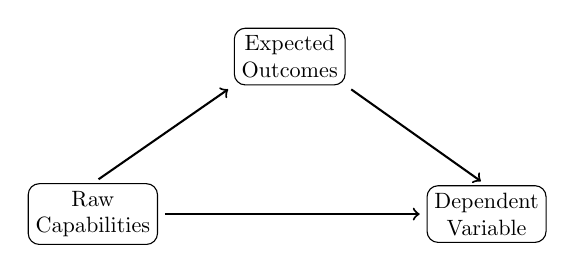
\begin{tikzpicture}[
  var/.style={
    rectangle,
    rounded corners,
    draw=black,
    align=center,
    scale=0.8
    }
  ]
  
  \node[var] (cap) at (0, 0) {Raw\\Capabilities};
  \node[var] (doe) at (2.5, 2) {Expected\\Outcomes};
  \node[var] (dv) at (5, 0) {Dependent\\Variable};

  \path[->, line width=0.75pt] (cap.north) edge[shorten <=0.25em, shorten >=0.25em] (doe.south west);
  \iftoggle{doe-to-dv}{\path[->, line width=0.75pt] (doe.south east) edge[shorten <=0.25em, shorten >=0.25em] (dv.north);}{}
  \iftoggle{cap-to-dv}{\path[->, line width=0.75pt] (cap.east) edge[shorten <=0.25em, shorten >=0.25em] (dv.west);}{}
\end{tikzpicture}

%%% Local Variables:
%%% mode: latex
%%% TeX-master: "doe"
%%% End:


  \caption{
    Raw capabilities only affect the outcome of interest through expectations.
  }
  \label{fig:dag-cap0-doe1}
\end{figure}

If theory suggests that material capabilities only affect the outcome of interest insofar as they shape expectations about how a dispute would end, then DOE scores are the best measure to control for.
Figure~\ref{fig:dag-cap0-doe1} contains a causal graph of this situation.
The clearest examples of theories where only expectations matter come from the formal literature on crisis bargaining.
Take \citeauthor{powell1999}'s~\citeyearpar{powell1999} theory of bargaining in the shadow of power.
War is possible only if the status quo distribution of benefits is far enough from the expected outcome of conflict that at least one state is dissatisfied.
An empirical model derived from this theory should control for DOE scores rather than the capability ratio or other poor proxies for expectations.

\begin{figure}[htp]
  \centering
  % Main document must include
% \usepackage{tikz}  % for the graphics
% \usepackage{etoolbox}  % for the if-then toggles

\providetoggle{cap-to-dv}
\providetoggle{doe-to-dv}

\toggletrue{cap-to-dv}
\toggletrue{doe-to-dv}

% Main document must include
% \usepackage{tikz}  % for the graphics
% \usepackage{etoolbox}  % for the if-then toggles

\providetoggle{cap-to-dv}
\providetoggle{doe-to-dv}

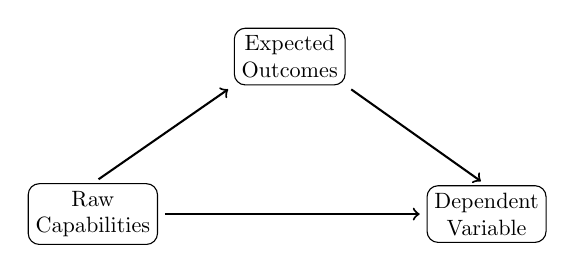
\begin{tikzpicture}[
  var/.style={
    rectangle,
    rounded corners,
    draw=black,
    align=center,
    scale=0.8
    }
  ]
  
  \node[var] (cap) at (0, 0) {Raw\\Capabilities};
  \node[var] (doe) at (2.5, 2) {Expected\\Outcomes};
  \node[var] (dv) at (5, 0) {Dependent\\Variable};

  \path[->, line width=0.75pt] (cap.north) edge[shorten <=0.25em, shorten >=0.25em] (doe.south west);
  \iftoggle{doe-to-dv}{\path[->, line width=0.75pt] (doe.south east) edge[shorten <=0.25em, shorten >=0.25em] (dv.north);}{}
  \iftoggle{cap-to-dv}{\path[->, line width=0.75pt] (cap.east) edge[shorten <=0.25em, shorten >=0.25em] (dv.west);}{}
\end{tikzpicture}

%%% Local Variables:
%%% mode: latex
%%% TeX-master: "doe"
%%% End:


  \caption{
    Raw capabilities affect the outcome of interest both directly and through expectations.
  }
  \label{fig:dag-cap1-doe1}
\end{figure}

If material capabilities affect the outcome both directly and indirectly via expectations, then it would be appropriate to control for both raw capabilities and expected dispute outcomes.
Figure~\ref{fig:dag-cap1-doe1} illustrates this scenario.
For example, imagine an empirical study of ``sinking costs'' via military mobilization in international crises \citep{fearon_signaling_1997}.
The initial movement of peaceful relations into a crisis, as well as early behavior at the bargaining table, might be shaped solely by states' expectations about dispute outcomes.
But if states build up their military as a way to signal resolve, independently of the effect on likely outcomes, then raw capabilities matter too.
When empirically modeling a theory like this, scholars should include both DOE scores and raw capability measures.
The ratio of CINC scores may or may not be the most appropriate way to capture raw capabilities---that, too, depends on the specifics of the theory.

\begin{figure}[htp]
  \centering
  % Main document must include
% \usepackage{tikz}  % for the graphics
% \usepackage{etoolbox}  % for the if-then toggles

\providetoggle{cap-to-dv}
\providetoggle{doe-to-dv}

\toggletrue{cap-to-dv}
\togglefalse{doe-to-dv}

% Main document must include
% \usepackage{tikz}  % for the graphics
% \usepackage{etoolbox}  % for the if-then toggles

\providetoggle{cap-to-dv}
\providetoggle{doe-to-dv}

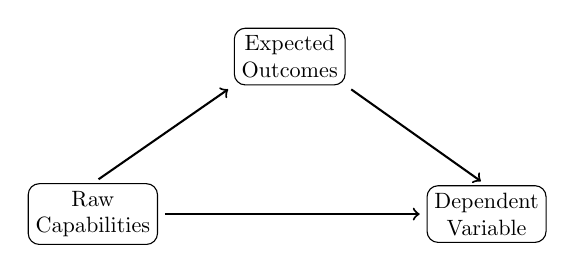
\begin{tikzpicture}[
  var/.style={
    rectangle,
    rounded corners,
    draw=black,
    align=center,
    scale=0.8
    }
  ]
  
  \node[var] (cap) at (0, 0) {Raw\\Capabilities};
  \node[var] (doe) at (2.5, 2) {Expected\\Outcomes};
  \node[var] (dv) at (5, 0) {Dependent\\Variable};

  \path[->, line width=0.75pt] (cap.north) edge[shorten <=0.25em, shorten >=0.25em] (doe.south west);
  \iftoggle{doe-to-dv}{\path[->, line width=0.75pt] (doe.south east) edge[shorten <=0.25em, shorten >=0.25em] (dv.north);}{}
  \iftoggle{cap-to-dv}{\path[->, line width=0.75pt] (cap.east) edge[shorten <=0.25em, shorten >=0.25em] (dv.west);}{}
\end{tikzpicture}

%%% Local Variables:
%%% mode: latex
%%% TeX-master: "doe"
%%% End:


  \caption{
    Raw capabilities directly affect the outcome of interest, but expectations do not.
  }
  \label{fig:dag-cap1-doe0}
\end{figure}

The last possibility to consider is that expectations do not affect the outcome of interest.
In this case, empirical models should only include raw capability measures, not DOE scores.
The clearest example is when the dispute outcome itself is the dependent variable.
First, absent some kind of self-fulfilling prophecy effect, we would expect actual capability holdings to drive outcomes more so than expectations.
Second, because DOE scores are calculated using the dispute outcome data, the DOE scores themselves are endogenous to observed outcomes, and thus should not be included as an independent variable when outcome is the dependent variable.\footnote{%
  In principle, this latter problem could be solved, albeit at great computational expense, by only using data for years up to $t-1$ to calculate the DOE score for year~$t$.
}

When there is no theory or the theory does not specify how material capabilities affect the outcome of interest, we recommend a data-driven approach.
The steps are the same ones we took in the replication analysis: determine a metric for model fit (whether in- or out-of-sample), run the model separately for each potential measure, and choose the best-fitting model.
Alternatively, if your theory says nothing about the relationship between capabilities and the outcome of interest, it may be best not to include capability measures at all.
A confounding variable, by definition, must be related to both the treatment and outcome of interest.
If raw capabilities are not supposed to affect the outcome either directly or through expectations, then they are not a confounder and there is no need to control for them.

%%% Local Variables:
%%% mode: latex
%%% TeX-master: "doe"
%%% End:



\section{Conclusion}
\label{sec:conclusion}

In this paper, we have argued that proxies should be constructed using predictive power as the criterion of interest, provided a method for doing so, and demonstrated the usefulness of the method in an application to measuring dispute outcomes.
We hope that our efforts will be of use both for the DOE scores we provide and for the theoretical merits of our general argument.

In our application, the DOE scores outperform the extant proxy---the CINC-based capability ratio---in a number of important ways.
In pure terms, the DOE score more closely relates to what international relations scholars care about: the expected outcome of a dispute between two nations.
It therefore has a more natural interpretation than the capability ratio.
It also lacks the \emph{ad hoc} assumptions imposed by both the CINC score and the ratio-based transformation used in most studies.
On the practical side, our replications suggest that the DOE score is a better contributor to the usual battery of variables included in the ever-expanding universe of international relations regressions.
We hope, then, that it will find use as scholars advance and test new claims. And, in a substantive sense, we find it interesting that our more flexible approach suggests that material capabilities play an important role in determining dispute outcomes.

Though it represents a massive improvement over the \emph{status quo}, the DOE score could still be improved.
We have only included those variables that could be extracted from the data used to construct the capability ratio---namely, the six Correlates of War National Material Capabilities variables.
We did so consciously, as we wanted to demonstrate that our method could improve measures without introducing new covariates.
Having made our point, we look forward to seeing what the future holds for coming versions of DOE when new data is brought to bear on the problem.
At the risk of belaboring: we created DOE using open-source software and have made our replication code available, and so anybody with a computer---and some patience!---could create a new version with new covariates.

On the theoretical side, we believe that our data-driven approach to measurement will prove useful for those wishing to proxy for other quantities.
All one needs is a set of predictor variables $\boldsymbol{x}$ and some outcome of interest $\boldsymbol{y}$---the $f$ we provide to map $\boldsymbol{x}$ to $\boldsymbol{y}$ will work.
Just as with introducing new covariates in any given application, future scholars can improve their proxies by including new models for evaluation in the super learner---the general approach remains unchanged.
Our application tasked us to create a proxy of a probabilistic expectation like those seen in formal models of choice under uncertainty, and similar applications provide a natural starting point for our method.
Doing so, however, requires good theory for just what it is that we hope to predict with our abstractions---for example, what outcome could we use variables related to democracy, like those used in the Polity score \citep{marshall2014}, to predict?
We hope political scientists across subfields will turn their attention to examples like these as they construct new measures and improve existing ones.

We would like to conclude with a still broader point.
\citet{Breiman:2001fd} argues that statistical modelers fall into one of two cultures: data modelers, who interpret models' estimates after assessing overall quality via in-sample goodness of fit; and algorithmic modelers, who seek algorithms that predict responses as well as possible given some set of covariates.\footnote{
  In case it is not obvious from our previous citations, Breiman self-identifies as an algorithmic modeler.
  He claims that 98\% of statisticians fall into the data modeling camp, or at least did as of 2001.
  We are comfortable positing that the percentage is similar, if not greater, for empirical political scientists in 2015.
}
The method we advance is certainly algorithmic.
Our decision to adopt algorithmic modeling based on prediction, however, was not culture-driven---it was purpose-driven \citep{clarke2012}.
Most simply, many quantities to be proxied for are expectations, so they should be constructed with prediction in mind.
But as we show in the replication analysis, an algorithmically constructed proxy can be useful to include in traditional models.
As new problems emerge and new solutions arise to solve them, we believe methodological pragmatism will be an important virtue.
We do not expect (nor encourage) empirical political science to turn its focus from causal hypothesis testing to prediction.
But good hypothesis testing depends on good measures, and sometimes the best way to build a measure is to assume the persona of the algorithmic modeler.
By doing just that, this paper has developed one measure that improves on the previous state of the art along a number of dimensions.

%%% Local Variables:
%%% mode: latex
%%% TeX-master: "doe"
%%% End:



\clearpage
\appendix
\section{Appendix}

\subsection{National Material Capabilities Data}

Our predictors are taken from the National Material Capabilities (v4.0) dataset from the Correlates of War project \citep{singer1972}.\footnote{
  Downloaded from \url{http://correlatesofwar.org/data-sets/national-material-capabilities/nmc-v4-data/at_download/file}.
}
The dataset contains observations on six variables for 14,199 country-years from 1816 to 2007.
For details on the variables and their measurement, see the NMC Codebook.\footnote{
  Available at \url{http://correlatesofwar.org/data-sets/national-material-capabilities/nmc-codebook/at_download/file}.
}
Table~\ref{tab:summary} lists the proportions of zeroes and missing values among each variable.

\begin{table}[htp]
  \centering
  \input{tab-summary}
  \caption{
    Proportions of zeroes and missing values in each National Military Capability component variable.
  }
  \label{tab:summary}
\end{table}

All six variables are strongly right-skewed.
Since five of the six variables are sometimes zero-valued (though all are non-negative), a logarithmic transformation is not appropriate.
Instead, to correct for skewness, we apply an inverse hyperbolic sine transformation \citep{Burbidge:1988gu} to each component:
\begin{equation}
  \label{eq:asinh}
  h(x, \theta)
  =
  \sinh^{-1} (\theta x)
  =
  \log \left(
    \theta x + \sqrt{(\theta x)^2 + 1}
  \right).
\end{equation}
We set the scale~$\theta$ separately for each component variable with the aim of making the transformed variable approximately normally distributed.
For each variable, we choose the value of $\theta \in \{2^d\}_{d=-10}^{10}$ that minimizes the Kolmogorov--Smirnov test statistic \citep{MasseyJr:2012jo} against a normal distribution with the same mean and variance.
Table~\ref{tab:summary} gives the scale selected for each component.
We use the transformed components in both the multiple imputation (see below) and the super learner training.

\subsection{Militarized Interstate Dispute Data}

Our sample and outcome variable are taken from the Militarized Interstate Disputes (v4.1) dataset from the Correlates of War project \citep{Palmer:2015hp}.\footnote{
  Downloaded from \url{http://correlatesofwar.org/data-sets/MIDs/mid-level/at_download/file}.
}
The dataset records the participants and outcomes of interstate disputes from 1816 to 2010.
To avoid the problem of aggregating capabilities across multiple states, we exclude disputes with more than one state on either side.
We drop disputes that end in an outcome other than one side winning, one side yielding, or a stalemate;\footnote{
  For details on other kinds of outcomes, see the MID Codebook.
}
we then collapse ``A Wins'' and ``B Yields'' into a single coding, and similarly for ``B Wins'' and ``A Yields.''
Finally, since the capabilities data only run through 2007, we exclude disputes that end after 2007.
In the end, we have $N = 1{,}740$ cases.

For each dispute in our dataset, we code the participating countries' capabilities using the values in the year the dispute began.
About 17~percent of disputes have at least one missing capability component for at least one participant.

\subsection{Multiple Imputation}

As noted above, all of the National Material Capabilities variables contain some missing values.
Following standard practice, we multiply impute the missing observations.
We perform the imputations via the \texttt{Amelia} software package \citep{pkg-Amelia}.

Rather than just impute the missing values in the final dataset of disputes, we impute the entire National Material Capabilities dataset.
This allows us to fully exploit the dataset's time-series cross-sectional structure in the imputation process \citep{honaker_what_2010}.
We include in the imputation model a cubic polynomial for time, interacted with country dummy variables.
As this results in an explosion in the number of parameters in the imputation model, we then impose a ridge prior equal to 0.1 percent of the observations in the dataset (see Section~4.7.1 of the \texttt{Amelia} package vignette).
We enforce the constraint that every imputed value be non-negative.
Finally, we impose an observation-level prior with mean zero and variance equal to that of the observed values of the corresponding component variable for every missing cell that meets the following criteria:
\begin{itemize}
  \item There are no non-zero observed values in the time series preceding the cell
  \item The first observed value that comes after the cell is zero
\end{itemize}
So, for example, if a country's urban population is zero from 1816 to 1840, missing from 1841 to 1849, and zero in 1850, we would impose this form of prior on the 1841--1849 values.
Diagnostic time series plots of observed versus imputed values within each data series, generated by the \texttt{tscsPlot()} function in \texttt{Amelia}, will be made available in the project's Dataverse.

The presence of missing data also complicates the calculations of country-by-country proportions of the total amount of each component by year.
One option is to recompute the annual totals in each imputed dataset, so that the resulting data will be logically consistent---in particular, all proportions will sum to one.
The drawback of this approach is that virtually every observation of the proportions will differ across the imputed datasets, even for countries with no missing data, since the annual totals will differ across imputations.
An alternative approach is to compute the annual totals using only the observed values.
The advantage is that non-missing observations will not vary across imputed datasets; the downside is that the proportions within each imputation will generally sum to more than one.
For our purposes in this paper, we think it is preferable to reduce variation across imputations, even at the expense of some internal consistency in the imputed datasets, so we take the latter approach: annual totals are the sums of only the observed values.

We impute $I = 10$ datasets of national capabilities according to the procedure laid out above, and we merge each with the training subset of our dispute data to yield $I$ training data imputations.
We run the super learner separately on each imputation, and our final model is an (unweighted) average of the $I$ super learners.

After training is complete, we run into missing data problems once again when calculating DOE scores.
To calculate predicted probabilities for dyads with missing values, we calculate a \emph{new} set of $I = 10$ imputations of the capabilities data and take an (unweighted) average of our model's predictions across the imputations.

\subsection{Super Learner Candidate Models}

We use the R statistical environment \citep{pkg-R} for all data analysis.
We fit, cross-validate, and calculate predictions from each candidate model through the \texttt{caret} package \citep{pkg-caret}.
We then construct the super learner by solving~\eqref{eq:super-learner} via base R's \texttt{constrOptim()} function for optimization with linear constraints.
Further details about each candidate model are summarized below.

\begin{itemize}
  \item Ordered Logit \citep{McKelvey:2010gv}
  \begin{description}
    \item[Package] \texttt{MASS} \citep{pkg-MASS}
    \item[Tuning Parameters] None
    \item[Notes] In the ``Year'' models, the year of the dispute is included directly and interacted with each capability variable
  \end{description}

  \item C5.0 \citep{Quinlan:2015uc}
  \begin{description}
    \item[Package] \texttt{C50} \citep{pkg-c50}
    \item[Tuning Parameters] ~
    \begin{itemize}
      \item Number of boosting iterations (\texttt{trials}): selected via cross-validation from $\{1, 10, 20, 30, 40, 50\}$
      \item Whether to decompose the tree into a rule-based classifier (\texttt{model}): selected via cross-validation
      \item Whether to perform feature selection (\texttt{winnow}): selected via cross-validation
    \end{itemize}
  \end{description}

  \item Support Vector Machine \citep{Cortes:1995ie}
  \begin{description}
    \item[Package] \texttt{kernlab} \citep{pkg-kernlab}
    \item[Tuning Parameters] ~
    \begin{itemize}
      \item Kernel width (\texttt{sigma}): selected via cross-validation from $\{0.2, 0.4, 0.6, 0.8, 1\}$
      \item Constraint violation cost (\texttt{C}): selected via cross-validation from $\{\frac{1}{4}, \frac{1}{2}, 1, 2, 4\}$
    \end{itemize}
    \item[Notes] Radial basis kernel
  \end{description}

  \item $k$-Nearest Neighbors \citep{Cover:1967jq}
  \begin{description}
    \item[Package] \texttt{caret} \citep{pkg-caret}
    \item[Tuning Parameters] ~
    \begin{itemize}
      \item Number of nearest neighbors to average (\texttt{k}): selected via cross-validation from $\{25, 50, \ldots, 250\}$
    \end{itemize}
    \item[Notes] All predictors centered and scaled to have zero mean and unit variance
  \end{description}

  \item CART \citep{Breiman:1984tu}
  \begin{description}
    \item[Package] \texttt{rpart} \citep{pkg-rpart}
    \item[Tuning Parameters] ~
    \begin{itemize}
      \item Maximum tree depth (\texttt{maxdepth}): selected via cross-validation from $\{2, 3, \ldots, 9, 10\}$ (only up to 9 for models without year included)
    \end{itemize}
  \end{description}

  \item Random Forest \citep{Breiman:2001fb}
  \begin{description}
    \item[Package] \texttt{randomForest} \citep{pkg-randomForest}
    \item[Tuning Parameters] ~
    \begin{itemize}
      \item Number of predictors randomly sampled at each split (\texttt{mtry}): selected via cross-validation from $\{2, 4, \ldots, 12\}$
    \end{itemize}
    \item[Notes] 1,000 trees per fit
  \end{description}

  \item Averaged Neural Nets \citep{Ripley:1996vd}
  \begin{description}
    \item[Package] \texttt{nnet} \citep{pkg-MASS}, \texttt{caret} \citep{pkg-caret}
    \item[Tuning Parameters] ~
    \begin{itemize}
      \item Number of hidden layer units (\texttt{size}): selected via cross-validation from $\{1, 3, 5, 7, 9\}$
      \item Weight decay parameter (\texttt{decay}): selected via cross-validation from $\{10^0, 10^{-1}, 10^{-2}, 10^{-3}, 10^{-4}\}$
    \end{itemize}
    \item[Notes] Creates an ensemble of 10 neural nets, each initialized with different random number seeds
  \end{description}
\end{itemize}

\subsection{Replications}

The following list contains basic information about each model in the replication study.
We carry out logistic and probit regressions via \texttt{glm()} in base R \citep{pkg-R}, multinomial logit via \texttt{multinom()} in the \texttt{nnet} package \citep{pkg-MASS}, ordered probit via \texttt{polr()} in the \texttt{MASS} package \citep{pkg-MASS}, and heteroskedastic probit via \texttt{hetglm()} in the \texttt{glmx} package \citep{pkg-glmx}.

\input{list-replications}

%%% Local Variables:
%%% mode: latex
%%% TeX-master: "doe"
%%% End:


\newpage
\bibliographystyle{apsr}
\bibliography{doebib}


\end{document}
